\documentclass{article}
\usepackage{enumitem}
\usepackage{amsmath}
\usepackage{graphicx}
\usepackage{url}
\title{Assignment-4}
\author{Name - Ajay Kanna, Roll No - AE22B024, Github id - Ajaykannaiitian}
\begin{document}
\maketitle
\section{AE22B024}
So here I am going to describe the continuity equation
\subsection{CONTINUITY EQUATION}
A continuity equation or transport equation is an equation that describes the transport of some quantity. It is particularly simple and powerful when applied to a conserved quantity
\subsection{integral form}
The integral form of the continuity equation states that:
\begin{itemize}
  \item The amount of q in a region increases when additional q flows inward through the surface of the region, and decreases when it flows outward.
  \item The amount of q in a region increases when new q is created inside the region, and decreases when q is destroyed.
  \item Apart from these two processes, there is no other way for the amount of q in a region to change.
Mathematically,
\end{itemize}
\begin{equation}
    \frac{dq}{dt} + \iint_S jdS = \Sigma
\end{equation}
\footnote{URL: \url{https://en.wikipedia.org/wiki/Continuity_equation}}
where,
\begin{itemize}
    \item S is any imaginary closed surface, that encloses a volume 
    \item q is the total amount of the quantity in the volume V
    \item j is the flux of q
    \item t is time
    \item $\Sigma$  is the net rate that q is being generated inside the volume V per unit time. When q is being generated, it is called a source of q, and it makes $\Sigma$ more positive. When q is being destroyed, it is called a sink of q, and it makes $\Sigma$ more negative
\end{itemize}
\cite{boris1976solution}
\footnote{URL: \url{https://en.wikipedia.org/wiki/Continuity_equation}}
\begin{figure}
    \centering
    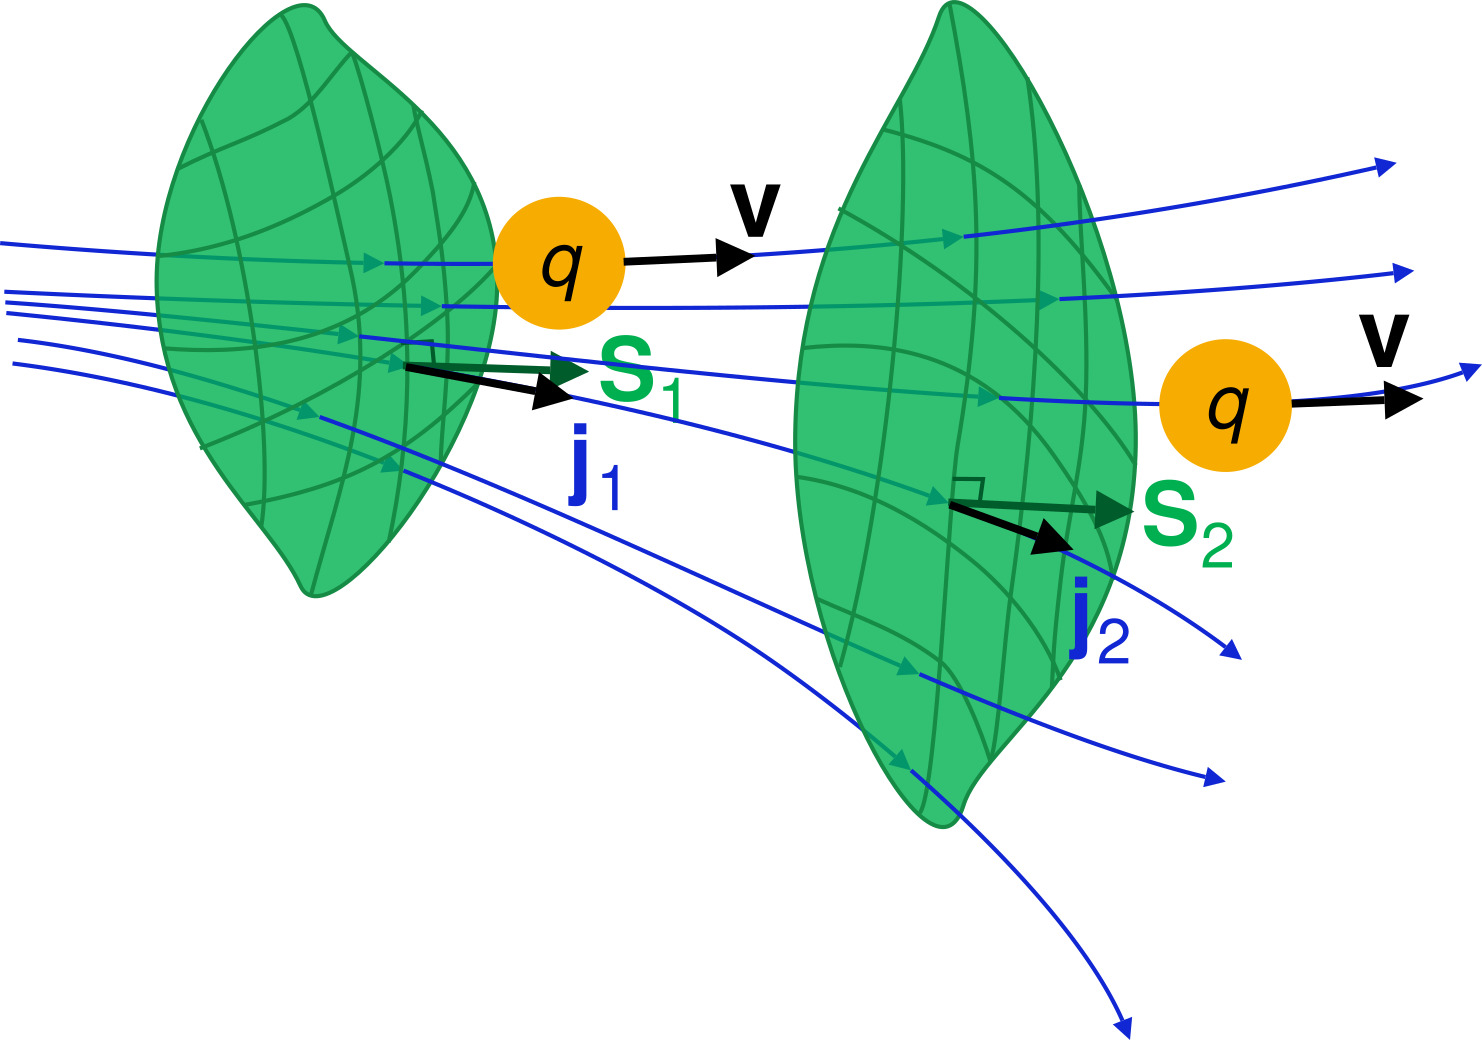
\includegraphics{Continuity_eqn_open_surface (1).jpg}
    \caption{Illustration of how the flux j of a quantity q passes through an open surface S}
    \label{fig:enter-label}
\end{figure}
\subsection{differential form}
\begin{equation}
    \frac{\partial \rho}{\partial t} + \nabla j = \sigma
\end{equation}
\cite{seis2017quantitative}
where,
\begin{itemize}
    \item $\rho$ is the amount of the quantity q per unit volume
    \item t is time
    \item j is the flux of q
    \item $\sigma$ is the generation of q per unit volume per unit time
\end{itemize}
This general equation may be used to derive any continuity equation, ranging from as simple as the volume continuity equation to as complicated as the Navier–Stokes equations. This equation also generalizes the advection equation.

In the case that q is a conserved quantity that cannot be created or destroyed (such as energy), $\sigma$ = 0 and the equations become:
\begin{equation}
    \frac{\partial \rho}{\partial t} + \nabla j = 0
\end{equation}
\cite{enwiki:1156826028}
\subsection{REASON FOR TAKING UP THE EQUATION:} 
Understanding and applying the continuity equation opens up a wide range of opportunities for analysis, design, research, and innovation in fields related to fluid dynamics. It forms the basis for solving real-world problems and advancing knowledge in various scientific and engineering disciplines.
\bibliographystyle{plain}
\bibliography{mybib}
\footnote{URL: \url{https://en.wikipedia.org/wiki/Continuity_equation}}
\end{document}
